%!TEX root = ../../main.tex
\section{Entity--Relationship Diagram}\label{sec:ERdiagram}
In order to have an idea of how the database handles bookings, location of bicycles, and their relation to the location of the stations, an ER Diagram was made, see \figref{fig:er-dia}.

\begin{figure}
	\centering
	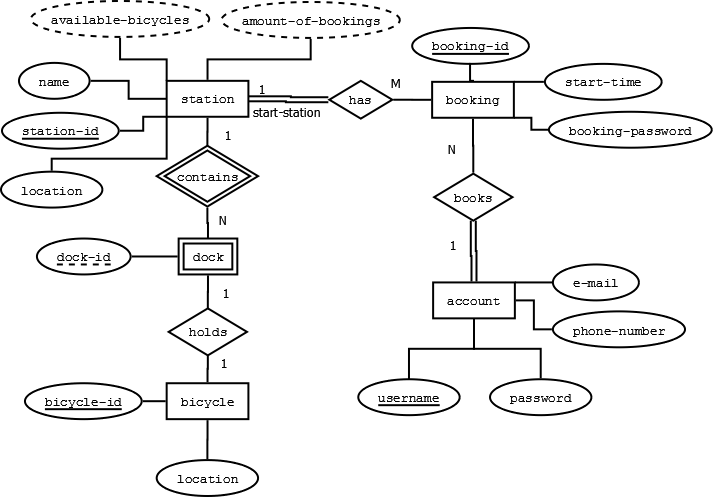
\includegraphics[scale=0.5, trim=0cm 0cm 7cm 0cm, clip]{relevantmaterial/erdiagram}
	\caption{The ER Diagram for database overview.}\label{fig:er-dia}
\end{figure}

As seen in the diagram, the entities consists of \texttt{bicycle}, \texttt{dock}, \texttt{station}, \texttt{booking}, and \texttt{account}.
An \texttt{account} consists of a \texttt{username}, \texttt{email}, which both must be unique, a \texttt{phone} number, \texttt{password} and a \texttt{role} which can be either a regular user or an administrator.
These attributes are common for an \texttt{account} entity, with the \texttt{phone} number being special in that the idea is that they should, in the future, be able to receive the booking password over SMS.

In relation to this is the \texttt{booking} entity, where it can be seen that a user can have many bookings whereas a booking is registered to one and only one account.
The \texttt{booking} then has a \texttt{booking_id}, to uniquely identify a booking, a \texttt{start_time}, such that a station knows when to lock a bicycle, and a password, used to unlock a bicycle if a correct password is entered in a time frame around the \texttt{start_time}.
Recall that the idea is that if a booking is not used in a given time frame at the \texttt{start_time}, the booking is removed, in order to free the bicycle for other to use.

A \texttt{booking} is also tied to a \texttt{station}, such that a \texttt{booking} is located at one and only one \texttt{station}, whereas a \texttt{station} can have many bookings.

A \texttt{booking} is also tied to a \texttt{bicycle}, such that when the booking is fulfilled it identifies which bicycle was taken.

A \texttt{station} has the attribute \texttt{station_id}, to uniquely identify the station.
Furthermore, it has a \texttt{name}, which is thought to be used to give a meaningful description of a given station.
We are aware that \texttt{name} could be used as a primary key, but having an integer id as the primary key reduce storage requirements when using foreign keys to the station id's.
%unlocks the possibility of duplicate names, which might be desired for stations located at different spots in the city, example could be two stations named "AAU Bycykel Station" which is a quite generic name.

In addition to this, a \texttt{station} has a \texttt{location}, which is used to easily place a station on a map, and can also be used for calculations such as distance between a given station and bicycle.
A \texttt{station} also has two derived attributes, which are \texttt{available_bicycles} and \texttt{amount_of_bookings}, where \texttt{available_bicycles} is beneficial to show to the user, such that they can see if it is possible to gather a bicycle at a given station.

Next is the \texttt{dock} entity, which is a weak entity, as it cannot exist without a \texttt{station}.
This represents the real-life situation with stations located around the city, and each of these has a number of docks.
The dock only has one attribute, which is the \texttt{dock_id}, used to identify a dock in combination with a \texttt{station_id}.

The interesting part of a \texttt{dock} is its relation with a \texttt{bicycle}.
A \texttt{dock} may or may not hold a \texttt{bicycle}, which is represented with the holds relation.

The \texttt{bicycle} entity then consists of a \texttt{bicycle_id}, to uniquely identify a given \texttt{bicycle}, and a \texttt{location}, which can be used to locate lost bicycles.

Keeping a log of information for administrative purposes as described in \secref{sec:designAdminTools}, requires additional database tables having timestamps as an important factor since the usage of bicycles is tied to some real life events that needs to be logged. 
In order to log the routes for a bicycle, a new relation is added to the database schema storing information about longitude and latitude and of course which bicycle it is for and when it was logged.
In order to log traffic of bicycles between stations another relation is added to the schema having information about a start station and an end station for a trip along with times for each of the events (start of trip and end of trip).
Last, a relation to store the count of bicycles at each station along with a timestamp, is added to the schema.

Putting all this together, also illustrating foreign key references, can be seen in \figref{fig:er-dia-log}.

\begin{figure}
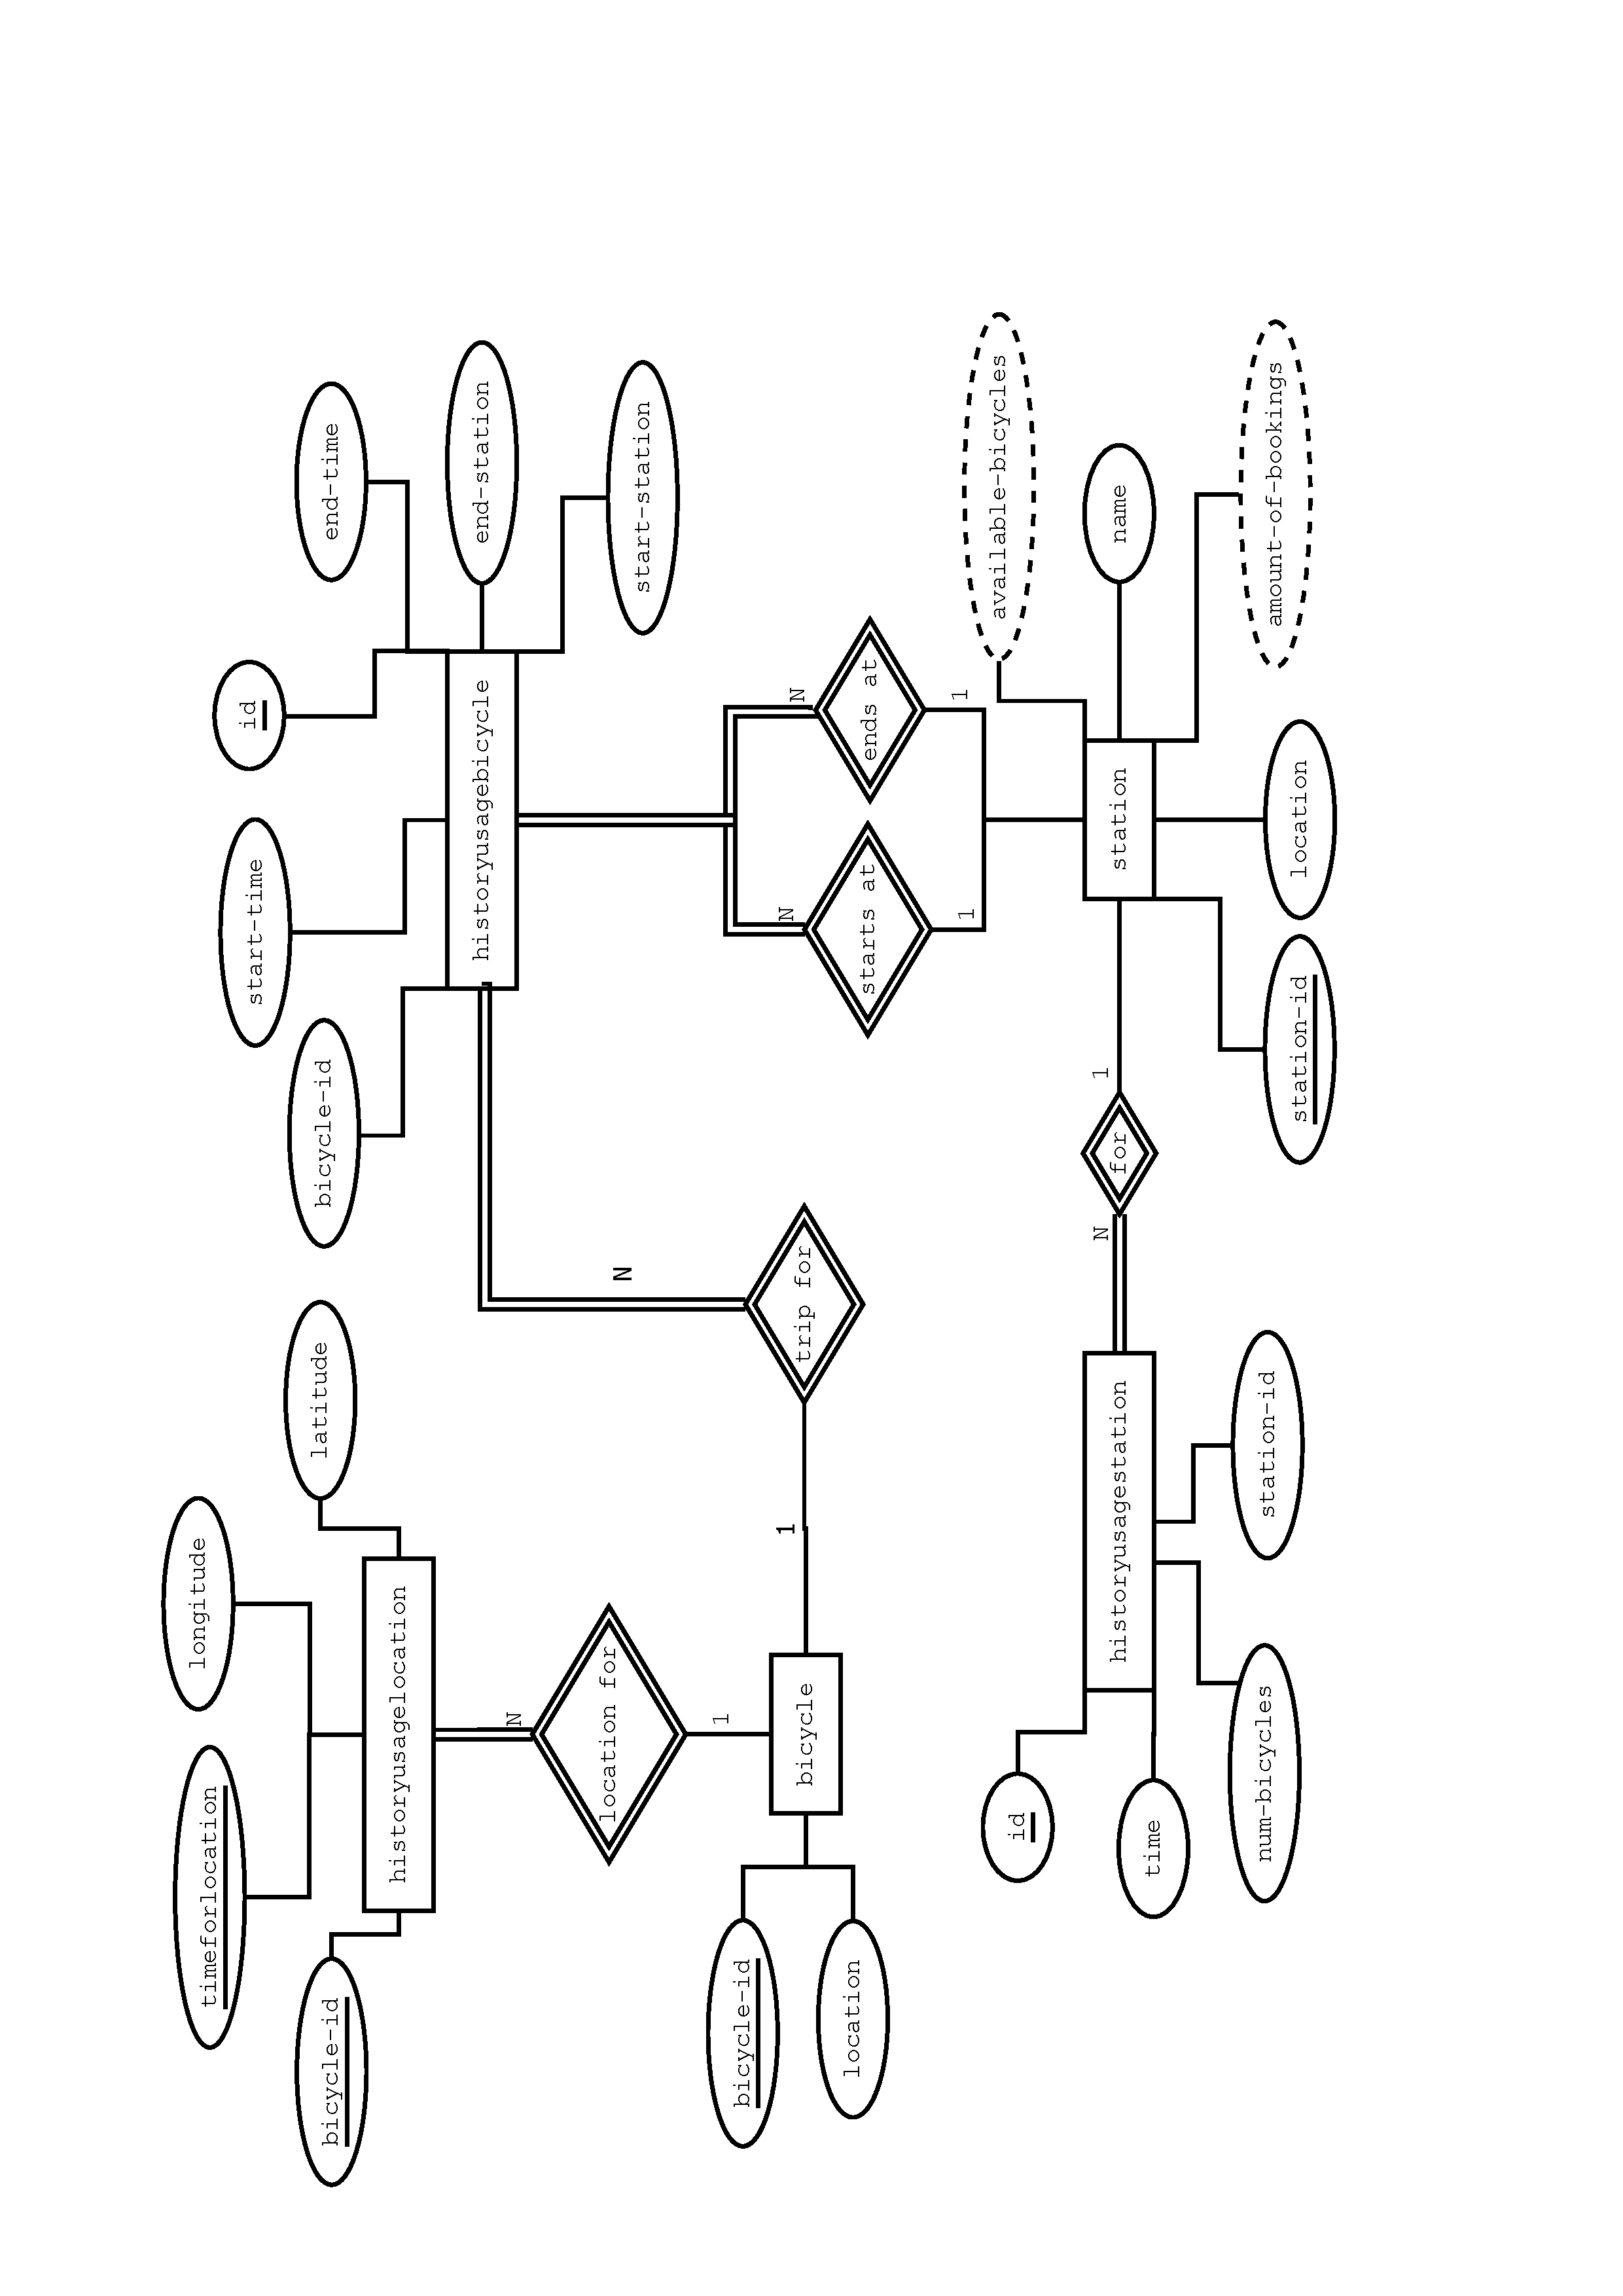
\includegraphics[scale=0.3, angle=-90]{design/ER-diagram-logging.pdf}
\vspace*{-2cm}
\caption{ER-diagram showing relations covering data logging.}\label{fig:er-dia-log}
\end{figure}

Addition and removal of bicycles, users, and stations is also part of the responsibility of the administration tools. 
For bicycles, they should be added to the system loosely and not directly to a station.
We intend to do it like this because when the administrator adds a new bicycle, they receive an id and the idea is that they use this id to program the bicycle such that it can be recognized by the system.
For users and stations, addition does not have any such considerations to make. 
The dock is not part of the administration tools, since it is handled at the stations.

Since the logging tables use the other tables like the station and bicycle tables it is important to handle deletion of stations and bicycles. 
If deletion is not handled properly the logged data could end up being inconsistent. 
In our case we handle deletion by adding a column to the affected tables indicating if the row is deleted or not, this ensures that we do not encounter foreign key constraints due to the logs referencing those rows. 
When using the station and bicycles table on the website we make sure to only use the rows that are not deleted, while for the history data we use all rows within a chosen time interval.
